\chapter{Architecture}
The architecture of each bounded context follows the Clean Architecture's structure: Entities, Use Cases, Interface Adapters, Frameworks and Drivers.

\begin{itemize}
    \item The first layer consists of the domain Aggregates we named Types; these are the domain entities and are the least likely to change when something external changes
    \item The second layer is composed of the domain ``Actions'', namely the business processes to model and ``Domain Events'': the starting point for almost all the business processes. They orchestrate the flow of data to and from the entities of the layer below
    \item For the Interface Adapters layer, in order to protect the layers underneath, we built Data Transfer Objects (DTOs) for every element that has to be transferred towards other bounded contexts or be persisted in storage. We also used the Repository pattern to abstract over the particular data persistence infrastructure. DTOs were also used in the Anti-Corruption Layer and Open-Host Service patterns to convert and present external data to the Entities and Use Case layers
    \item As for the Frameworks and Drivers layer, it contains the minimal amount of code needed to glue together the ``communication code'' (HTTP servers, Database persistence, etc.) with the code below. We implemented the HTTP servers belonging to this layer and mocked the remaining code related to data persistence or message-oriented communication.
    
    However, we did not mock the code necessary to communicate with the digital twins.
    We allowed the transfer of information with the usage of WebSockets, so we could receive data and events sent directly from the digital twins.
\end{itemize}


\begin{figure}[H]
    \centering
    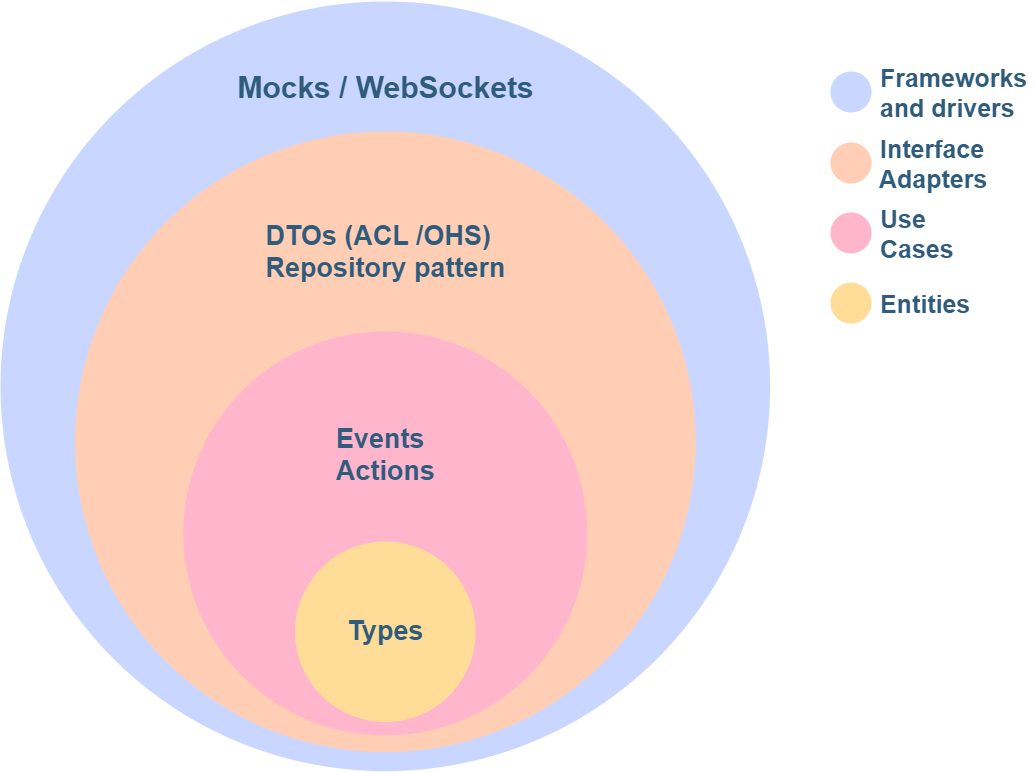
\includegraphics[width=0.8\textwidth]{img/clean-architecture.png}
    \caption{Bounded Contexts architecture}
    \label{img:clean-architecture}
\end{figure}

\section{Context Map}
In this chapter, we analyzed the bounded contexts related to digital twins and their relationships.
The context map in figure \ref{img:context-map} represents the relationships patterns between the bounded contexts.

\begin{itemize}
    \item \textbf{MilkPlanning [D, ACL] $\leftarrow$ [U] MilkTankDT}
    
    \texttt{MilkPlanning} receives the information about the tanks' milk quantity from the \texttt{MilkTankDT}.
    \texttt{MilkPlanning} is a downstream bounded context and has an Anti-Corruption Layer.
    
    \item \textbf{Stocking [D, ACL] $\leftarrow$ [U] PackagingMachineDT \\ 
    Stocking [D, ACL] $\leftarrow$ [U] ScaleDT \\ 
    Stocking [D, ACL] $\leftarrow$ [U] MetalDetectorDT}

    \texttt{Stocking} receives the information about the quality assurance status considering the packaging machine, scale and metal detector. Data are sent from the \texttt{PackagingMachineDT}, \texttt{ScaleDT} and \texttt{MetalDetectorDT} respectively.
    \texttt{Stocking} is a downstream bounded context and has an Anti-Corruption Layer.
	
	\item \textbf{Alert [D, ACL] $\leftarrow$ [U] MilkTankDT \\
	Alert [D, ACL] $\leftarrow$ [U] MetalDetectorDT \\
	Alert [D, ACL] $\leftarrow$ [U]PackagingMachineDT \\
	Alert [D, ACL] $\leftarrow$ [U]ScaleDT}

    \texttt{Alert} receives the alerting messages from the digital twins. Data are sent from the \texttt{MilkTankDT}, \texttt{MetalDetectorDT}, \texttt{PackagingMachineDT} and \texttt{ScaleDT} respectively.
    \texttt{Alert} is a downstream bounded context and has an Anti-Corruption Layer.

    \item \textbf{MilkPlanning [D, ACL] $\leftarrow$  [U] Stocking} 
    
    \texttt{MilkPlanning} asks \texttt{Stocking} for the amount of products in stock.
    \texttt{MilkPlanning} is a downstream bounded context and has an Anti-Corruption Layer.

    \item \textbf{Alert[D, ACL] $\leftarrow$  [U] Maintenance}
    
    \texttt{Maintenance} sends the alerting messages about machine failure to \texttt{Alert}.
    \texttt{Alert} is a downstream bounded context and has an Anti-Corruption Layer.

	\item \textbf{Maintenance[D, ACL] $\leftarrow$  [U] PackagingMachineDT}
	
    \texttt{Maintenance} receives the information about the packaging machine status from \texttt{PackagingMachineDT} in order to forecast packaging machine failures.
    \texttt{Maintenance} is a downstream bounded context and has an Anti-Corruption Layer.

	\item \textbf{Reporting[D] $\leftarrow$  [U] ScaleDT \\
    Reporting[D] $\leftarrow$  [U] MetalDetectorDT }

    \texttt{Reporting} receives information from \texttt{ScaleDT} and \texttt{MetalDetectorDT} about their status in order to generate reports.
	

\end{itemize}

\begin{figure}[H]
    \centering
    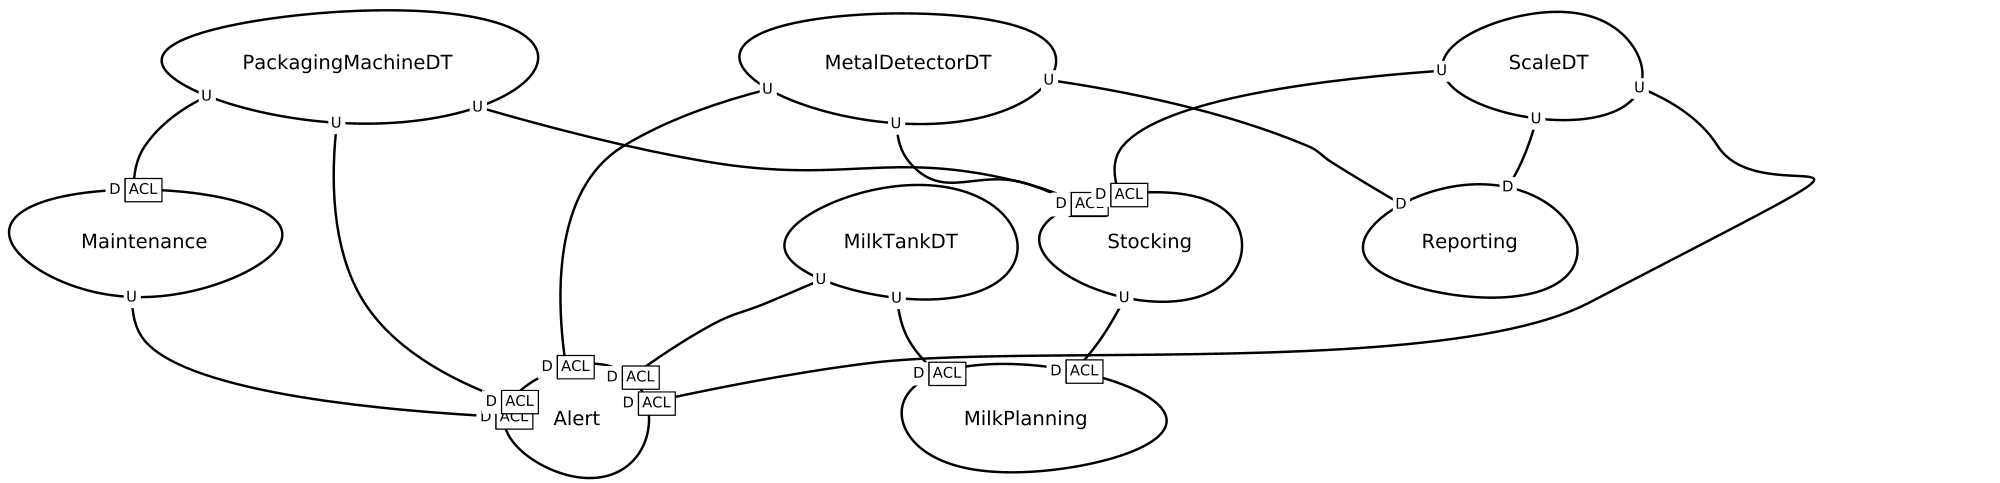
\includegraphics[width=\textwidth]{img/context-map.png}
    \caption{Context Map}
    \label{img:context-map}
\end{figure}


